\section{행동모형 결과}
\label{sec:behavioral-results}

이 절은 단승가격과 실현 착순으로 다른 연도에서 추정한 확률모형과 가중함수를
검증연도의 전체 가격벡터에 고정하여 적용한 결과다. 순서형 쌍승·삼쌍승은
M-R과 M-S2/M-S3의 직접 식별에 사용하고, 순서 없는 복승·삼복승은 모형을
다시 맞추지 않는 외부검증으로 남긴다. 모든 가격비교는 해당 승식의 전체
배당벡터가 비검열인 경주만 사용한다.

\subsection{조건부 순위확률의 표본 밖 검증}

\begin{table}[htbp]
\centering
\caption{연도 밖 조건부 순위확률 검증. ECE는 각 검증연도에서 계산한
10-bin calibration error의 경주수 가중평균이며 퍼센트포인트로 표시한다.}
\label{tab:behavioral-rank-validation}
\resizebox{0.92\textwidth}{!}{\begin{tabular}{llrrr}
\toprule
단계 & 확률모형 & 검증경주 & 평균 로그손실 & 평균 fold ECE \\
\midrule
1위 & 보정 Harville($\alpha=1$) & 19,301 & 1.7741 & 0.37\% \\
1위 & 보정·단계조정 & 19,301 & 1.7741 & 0.37\% \\
2위$\mid$1위 & 보정 Harville($\alpha=1$) & 19,301 & 1.9352 & 1.96\% \\
2위$\mid$1위 & 보정·단계조정 & 19,301 & 1.9066 & 0.42\% \\
3위$\mid$1·2위 & 보정 Harville($\alpha=1$) & 19,301 & 1.9722 & 3.29\% \\
3위$\mid$1·2위 & 보정·단계조정 & 19,301 & 1.8999 & 0.60\% \\
\bottomrule
\end{tabular}
}
\end{table}

\begin{figure}[htbp]
\centering
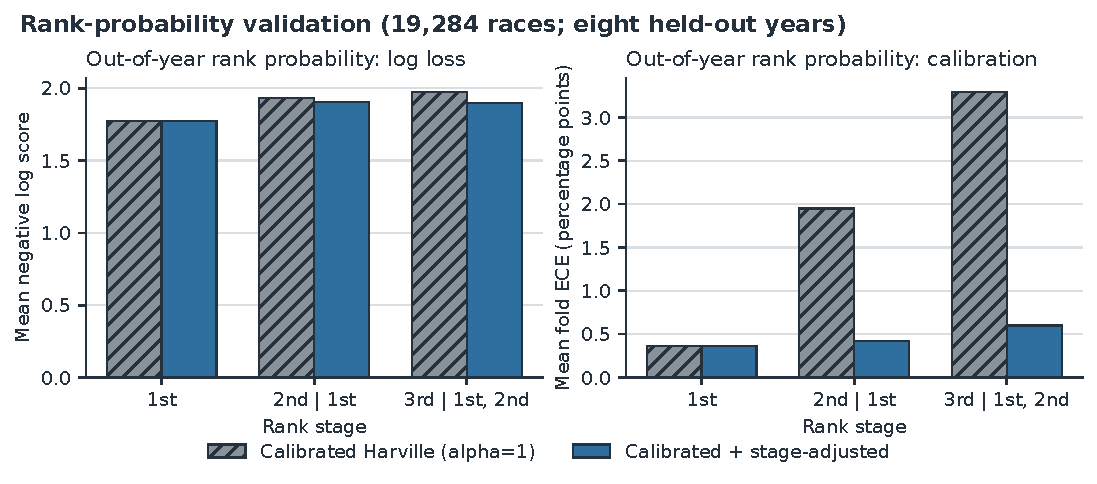
\includegraphics[width=0.96\textwidth]{figures/calibration-rank-probabilities.pdf}
\caption{조건부 순위확률의 연도 밖 로그손실과 보정오차}
\label{fig:behavioral-rank-validation}
\end{figure}

표~\ref{tab:behavioral-rank-validation}에서 1위 확률은 두 모형이 같고, 차이는
2·3위의 조건부 단계에서 생긴다. 단계조정 모형은 Harville 대비 2위 로그손실을
1.47\%, 3위 로그손실을 3.66\% 낮춘다. 평균 fold ECE도 2위에서
1.95에서 0.42 퍼센트포인트로, 3위에서 3.29에서 0.60 퍼센트포인트로
감소한다. 남은 선택집합이 10마리일 때 단계 온도계수는 여덟 fold에서 2위
0.729--0.746, 3위 0.565--0.579 범위다. 따라서 이하의 행동모형 비교는
실현 착순을 설명하지 못하는 임의의 Harville 입력이 아니라, 연도 밖에서
검증된 단계조정 순위확률을 선호 명세로 사용한다.

\subsection{순서형 가격벡터의 축약과 순차평가}

\begin{table}[htbp]
\centering
\caption{선호 명세의 행동가격모형 비교. 단계조정 순위확률과 Prelec
가중함수를 사용한다. 공통지지는 각 청구권의 모든 가중함수 인수가 훈련 단승확률의
1--99백분위 안에 드는 비율이다. M-U는 비모수적으로 회수하면 M-R과
관측적으로 같으므로 생략한다.}
\label{tab:behavioral-model-comparison}
\resizebox{0.88\textwidth}{!}{\begin{tabular}{llrrrr}
\toprule
시장 & 모형 & 경주수 & 중앙 TV & 중앙 로그 RMSE & 공통지지 \\
\midrule
쌍승 & M-R & 18,720 & 0.2534 & 1.0149 & 69.5\% \\
쌍승 & M-S2 & 18,720 & 0.1263 & 0.4548 & 98.0\% \\
\addlinespace
삼쌍승 & M-R & 3,323 & 0.3179 & 0.9778 & 38.1\% \\
삼쌍승 & M-S2 & 3,323 & 0.2075 & 0.5633 & 98.0\% \\
삼쌍승 & M-S3 & 3,323 & 0.1577 & 0.4728 & 98.9\% \\
\addlinespace
복승 & M-R & 19,286 & 0.1834 & 0.8097 & 81.4\% \\
복승 & M-S2 & 19,286 & 0.1300 & 0.4521 & 96.1\% \\
\addlinespace
삼복승 & M-R & 15,864 & 0.2775 & 1.0444 & 63.9\% \\
삼복승 & M-S2 & 15,864 & 0.2204 & 0.7217 & 74.8\% \\
삼복승 & M-S3 & 15,864 & 0.1545 & 0.5185 & 96.5\% \\
\bottomrule
\end{tabular}
}
\end{table}

\begin{figure}[htbp]
\centering
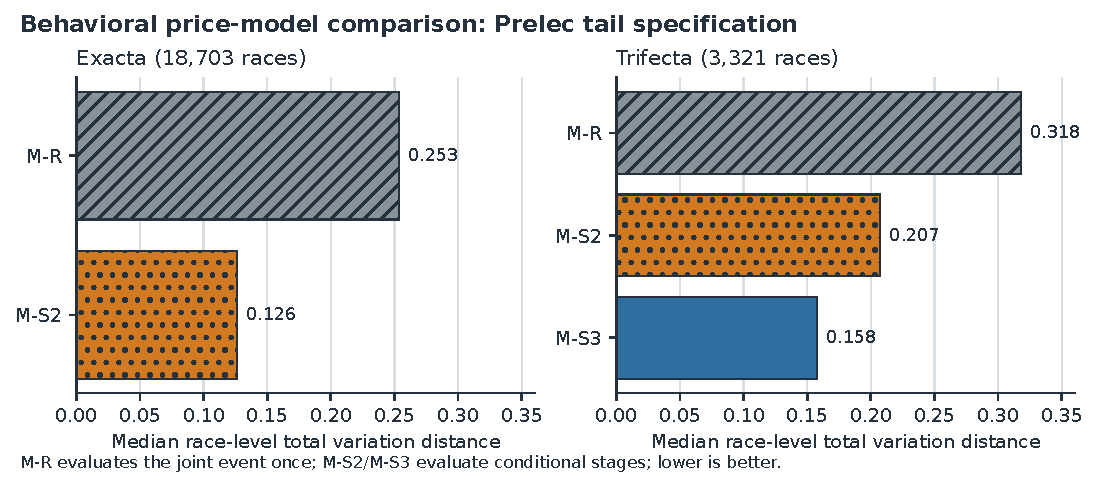
\includegraphics[width=0.96\textwidth]{figures/model-comparison-behavioral.pdf}
\caption{순서형 승식의 행동가격모형 TV 비교}
\label{fig:behavioral-ordered-comparison}
\end{figure}

쌍승에서 경주별 TV 중앙값은 M-R의 0.2534에서 M-S2의 0.1264로
낮아진다. 짝지은 개선폭 중앙값은 0.1230이고, 999회 경주일 군집
bootstrap 95\% 구간은 [0.1220, 0.1243]이다. 삼쌍승에서는 M-R
0.3178, M-S2 0.2075, M-S3 0.1578 순이다. M-R 대비 M-S3의
개선폭 중앙값은 0.1554[0.1533, 0.1577]이고, M-S2 대비 세 번째
단계를 분리했을 때에도 0.0498[0.0485, 0.0511]만큼 낮아진다.
이 네 비교의 연도별 TV 개선 중앙값은 모두 8개 연도에서 양수다.

이 결과가 하나의 손실함수에만 의존하는 것은 아니다. JS에서도 같은 순위를
얻고, 끝점 고정 isotonic 명세와 Prelec 명세의 TV 방향도 일치한다. 다만
삼쌍승 M-S3의 M-S2 대비 로그 RMSE 개선은 Prelec 명세에서 8개 연도 중
6개, isotonic 명세에서 5개 연도에서만 양수다. 따라서 세 번째 평가단계가
모든 손실함수와 모든 연도를 지배한다고 표현하지 않고, TV와 JS에서 일관된
우위라고 제한한다. power 명세에서는 순서형 M-R·M-S2·M-S3의 TV가
기계정밀도 수준에서 일치하여, 곱셈적 가중함수의 축약 불변성이 예상대로
재현된다.

\subsection{복승·삼복승의 무순서 외부검증}

\begin{figure}[htbp]
\centering
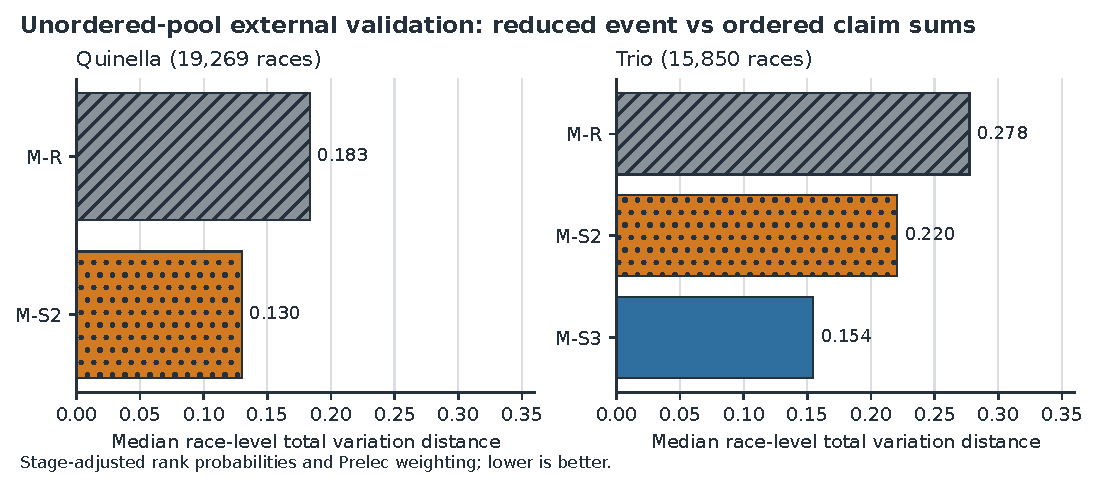
\includegraphics[width=0.96\textwidth]{figures/model-comparison-unordered.pdf}
\caption{무순서 승식의 외부검증: 결합사건의 축약평가와 순서형 청구권
예측가격 합의 비교}
\label{fig:behavioral-unordered-comparison}
\end{figure}

\begin{table}[htbp]
\centering
\caption{선호 명세의 짝지은 TV 개선폭. 구간은 경주일을 군집으로 999회
재표집한 개별 95\% bootstrap 구간이며 다중비교 보정을 적용하지 않았다.}
\label{tab:behavioral-model-improvements}
\resizebox{\textwidth}{!}{\begin{tabular}{lllrrr}
\toprule
시장 & 기준 & 비교모형 & TV 개선 중앙값 & 95\% 구간 & 양의 연도 \\
\midrule
쌍승 & M-R & M-S2 & 0.1230 & [0.1220, 0.1243] & 8/8 \\
\addlinespace
삼쌍승 & M-R & M-S2 & 0.1069 & [0.1049, 0.1082] & 8/8 \\
삼쌍승 & M-R & M-S3 & 0.1554 & [0.1533, 0.1577] & 8/8 \\
삼쌍승 & M-S2 & M-S3 & 0.0498 & [0.0485, 0.0511] & 8/8 \\
\addlinespace
복승 & M-R & M-S2 & 0.0557 & [0.0544, 0.0569] & 8/8 \\
\addlinespace
삼복승 & M-R & M-S2 & 0.0543 & [0.0538, 0.0548] & 8/8 \\
삼복승 & M-R & M-S3 & 0.1213 & [0.1201, 0.1228] & 8/8 \\
삼복승 & M-S2 & M-S3 & 0.0663 & [0.0654, 0.0675] & 8/8 \\
\bottomrule
\end{tabular}
}
\end{table}

순서 없는 풀에서도 같은 방향이 유지된다. 복승의 TV 중앙값은 결합확률합을
한 번 평가하는 M-R에서 0.1833이고, 두 쌍승 순서의 M-S2 청구권 가격을
합하면 0.1300이다. 짝지은 개선폭은 0.0557[0.0544, 0.0569]이며
8개 연도 모두 양수다. 삼복승은 M-R 0.2775, 여섯 삼쌍승 순서의 M-S2 합
0.2204, M-S3 합 0.1545 순이다. M-R 대비 M-S3 개선폭은
0.1213[0.1201, 0.1228], M-S2 대비 M-S3 개선폭은
0.0663[0.0654, 0.0675]이고 두 비교 모두 8개 연도에서 양수다.
복승·삼복승에서는 로그 RMSE와 JS도 같은 연도별 방향을 보인다.

이 검정은 무순서 승식에 자의적인 첫 번째 말을 지정한 결과가 아니다. M-R은
두 순서 또는 여섯 순서의 객관확률을 먼저 합한 뒤 $w$를 한 번 적용한다.
M-S2와 M-S3은 각 순서형 청구권의 단계별 점수를 계산한 뒤 그 청구권 가격을
합한다. 따라서 순서형 풀에서 식별한 비축약 표현이 별도 무순서 풀의 전체
가격벡터로 이동하는지를 묻는 진정한 leave-one-pool-out 외부검증이다.

\subsection{과거 자료만 사용하는 시간순 검증}

연도 제외 교차적합은 검증연도보다 뒤의 자료도 훈련에 사용할 수 있다. 이를
배제하기 위해 2017년부터 각 검증연도 직전까지의 자료만 누적하여 같은 모형을
다시 추정했다. 2016년은 이전 훈련연도가 없으므로 시간순 검증에서 제외한다.
이 expanding-window 표본은 착순확률 17,745개 경주, 쌍승 17,324개,
삼쌍승 3,130개, 복승 17,736개와 삼복승 14,840개 비검열 경주를 포함한다.

시간순 검증에서도 단계조정 모형의 로그손실은 Harville 대비 2위에서 1.47\%,
3위에서 3.65\% 낮다. 이는 앞서 보고한 19,284개 경주의 연도제외 3.66\%와
달리, 17,745개 경주의 과거연도 전용 표본에서 얻은 별도 추정치다. 선호 명세의
TV 중앙값은 쌍승에서 M-R 0.2664와
M-S2 0.1326, 삼쌍승에서 M-R 0.3258, M-S2 0.2143과 M-S3
0.1596이다. 복승은 0.1955와 0.1341, 삼복승은 0.2906, 0.2317과
0.1599 순이다. 표~\ref{tab:behavioral-time-forward}의 여덟 TV 대비는
모두 7개 시간순 검증연도에서 같은 방향을 유지한다.

\begin{table}[htbp]
\centering
\caption{과거 연도만 훈련에 사용한 시간순 검증의 짝지은 TV 개선폭. 구간은
경주일을 군집으로 999회 재표집한 개별 95\% bootstrap 구간이며 다중비교
보정을 적용하지 않았다.}
\label{tab:behavioral-time-forward}
\resizebox{\textwidth}{!}{\begin{tabular}{lllrrr}
\toprule
시장 & 기준 & 비교모형 & TV 개선 중앙값 & 95\% 구간 & 양의 연도 \\
\midrule
쌍승 & M-R & M-S2 & 0.1305 & [0.1291, 0.1318] & 7/7 \\
\addlinespace
삼쌍승 & M-R & M-S2 & 0.1073 & [0.1057, 0.1087] & 7/7 \\
삼쌍승 & M-R & M-S3 & 0.1615 & [0.1590, 0.1635] & 7/7 \\
삼쌍승 & M-S2 & M-S3 & 0.0534 & [0.0523, 0.0548] & 7/7 \\
\addlinespace
복승 & M-R & M-S2 & 0.0656 & [0.0642, 0.0672] & 7/7 \\
\addlinespace
삼복승 & M-R & M-S2 & 0.0559 & [0.0555, 0.0564] & 7/7 \\
삼복승 & M-R & M-S3 & 0.1294 & [0.1278, 0.1307] & 7/7 \\
삼복승 & M-S2 & M-S3 & 0.0721 & [0.0711, 0.0730] & 7/7 \\
\bottomrule
\end{tabular}
}
\end{table}

\subsection{공통지지와 식별의 한계}

\begin{figure}[htbp]
\centering
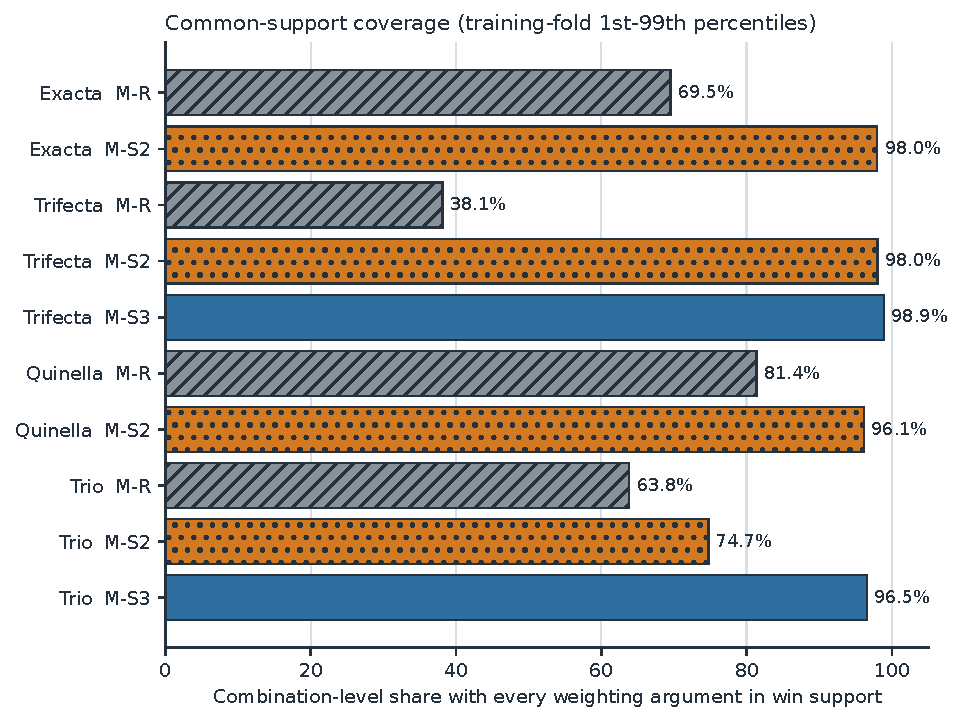
\includegraphics[width=0.92\textwidth]{figures/model-comparison-support.pdf}
\caption{훈련 단승확률 공통지지에 포함되는 가중함수 인수의 비율}
\label{fig:behavioral-support}
\end{figure}

% Source: outputs/behavioral_model_comparison.csv,
% probability_model=stage_temperature, tail_model=prelec, price_model=M-R,
% columns mean_support_share and all_arguments_supported_race_share.
M-R의 평균 공통지지는 쌍승 69.5\%, 삼쌍승 38.1\%, 복승 81.4\%,
삼복승 63.9\%다. M-S2는 각각 98.0\%, 98.0\%, 96.1\%, 74.7\%이고,
M-S3은 삼쌍승 98.9\%, 삼복승 96.5\%다. 더 엄격하게 한 경주의 모든 조합이
공통지지 안에 있는지를 보면 M-R의 비율은 쌍승 3.4\%, 삼쌍승 0.09\%,
복승 13.2\%, 삼복승 1.5\%에 그친다. 특히 희박한 결합확률을 한 번에
평가하는 M-R의 절대오차는 단승에서 관찰하지 못한 꼬리 외삽에 더 민감하다.
그러므로 선호 Prelec 명세의 절대 TV만으로 모형을 선택하지 않고, 공통지지를
명시한 isotonic 끝점 명세의 같은 방향과 power 음성대조를 함께 판정한다.

종합하면, 결과는 순서형·무순서형 네 승식 모두에서 복합사건의 완전 축약보다
조건부 순위단계를 분리한 가격표현과 더 잘 양립한다. 삼쌍승과 삼복승에서는
세 번째 단계를 별도로 평가한 M-S3이 TV 기준으로 추가 설명력을 갖는다.
그러나 M-U와 M-R은 단승 가격만으로 관측적으로 동등하고, 풀별 참가자 구성과
유동성도 관찰되지 않는다. 따라서 이 결과를 대표적 가격함수의 안정적인
비축약 표현에 대한 증거로 해석하되, 모든 개인의 확률오인이나 특정 인지과정을
직접 식별한 결과로 확대하지 않는다.
